% Created by tikzDevice version 0.12 on 2018-11-08 15:03:43
% !TEX encoding = UTF-8 Unicode
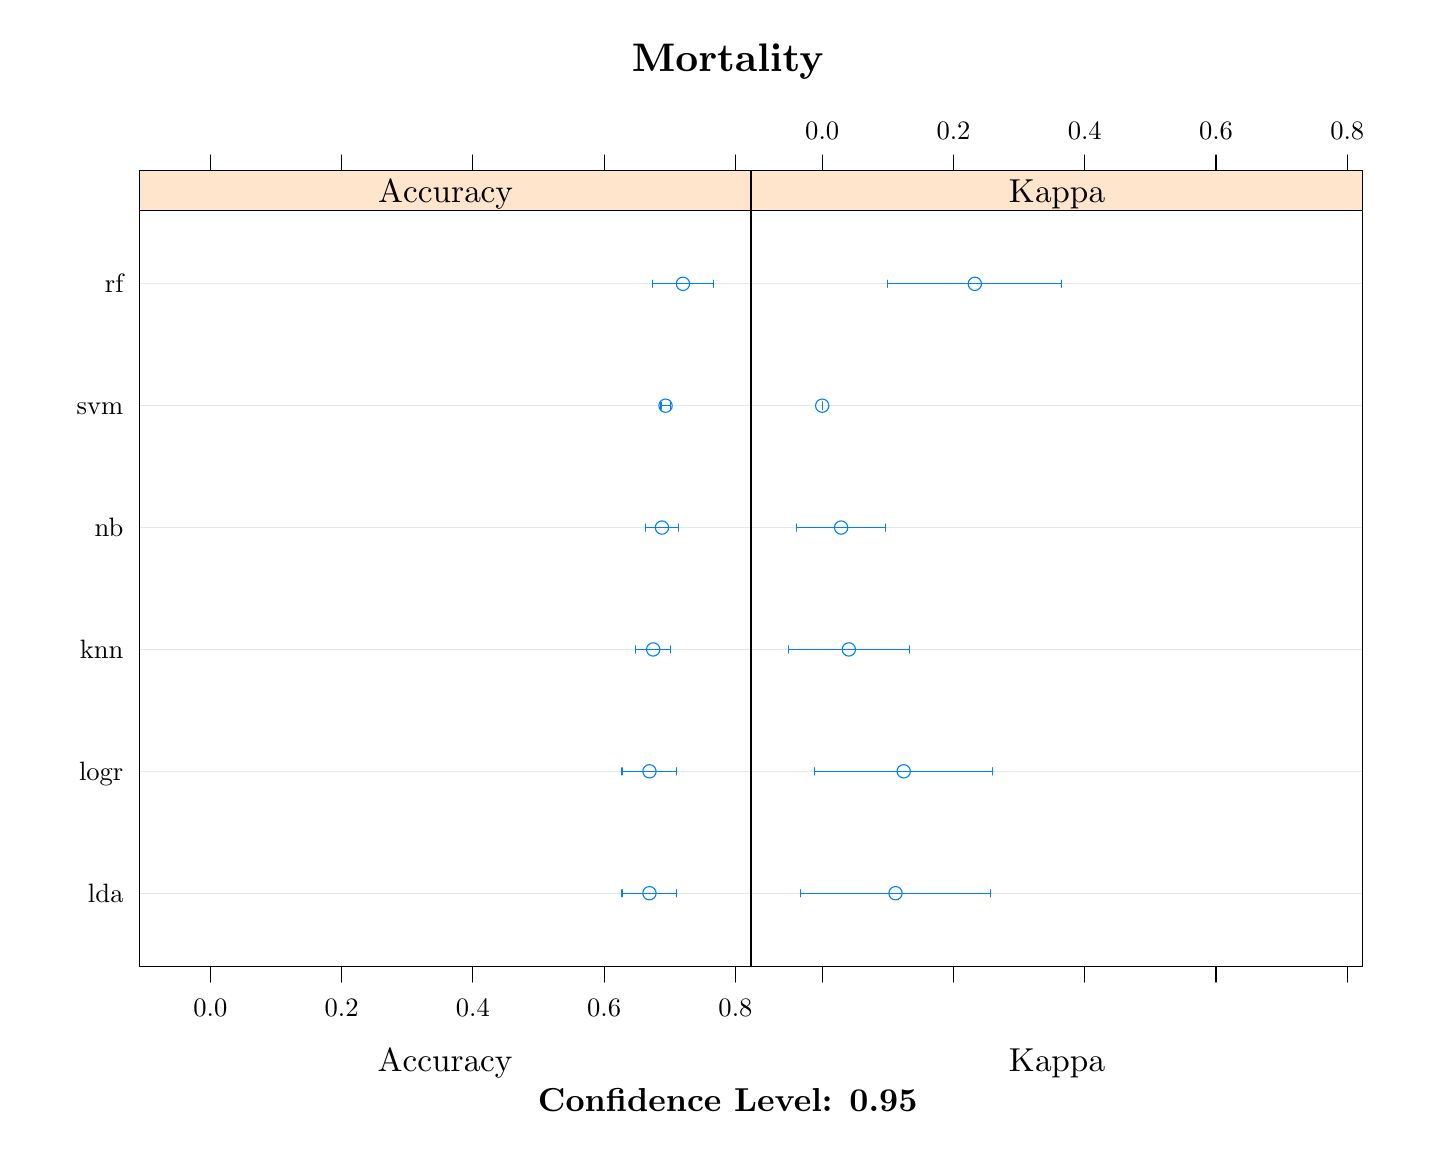
\begin{tikzpicture}[x=1pt,y=1pt]
\definecolor{fillColor}{RGB}{255,255,255}
\path[use as bounding box,fill=fillColor,fill opacity=0.00] (0,0) rectangle (505.89,397.48);
\begin{scope}
\path[clip] (  0.00,  0.00) rectangle (505.89,397.48);

\path[] (  0.00,  0.00) rectangle (505.89,397.48);
\definecolor{drawColor}{RGB}{0,0,0}

\node[text=drawColor,anchor=base,inner sep=0pt, outer sep=0pt, scale=  1.44] at (252.94,381.52) {\bfseries Mortality};
\end{scope}
\begin{scope}
\path[clip] (  0.00,  0.00) rectangle (505.89,397.48);
\definecolor{drawColor}{RGB}{0,0,0}

\node[text=drawColor,anchor=base,inner sep=0pt, outer sep=0pt, scale=  1.20] at (252.94,  6.02) {\bfseries Confidence Level: 0.95};
\end{scope}
\begin{scope}
\path[clip] (  0.00,  0.00) rectangle (505.89,397.48);
\definecolor{drawColor}{RGB}{0,0,0}

\node[text=drawColor,anchor=base,inner sep=0pt, outer sep=0pt, scale=  1.20] at (150.82, 20.33) {Accuracy};

\node[text=drawColor,anchor=base,inner sep=0pt, outer sep=0pt, scale=  1.20] at (371.92, 20.33) {Kappa};
\end{scope}
\begin{scope}
\path[clip] (  0.00,  0.00) rectangle (505.89,397.48);
\definecolor{drawColor}{RGB}{0,0,0}

\path[draw=drawColor,line width= 0.4pt,line join=round,line cap=round] ( 66.02,345.80) -- ( 66.02,351.49);

\path[draw=drawColor,line width= 0.4pt,line join=round,line cap=round] (113.45,345.80) -- (113.45,351.49);

\path[draw=drawColor,line width= 0.4pt,line join=round,line cap=round] (160.89,345.80) -- (160.89,351.49);

\path[draw=drawColor,line width= 0.4pt,line join=round,line cap=round] (208.32,345.80) -- (208.32,351.49);

\path[draw=drawColor,line width= 0.4pt,line join=round,line cap=round] (255.76,345.80) -- (255.76,351.49);
\end{scope}
\begin{scope}
\path[clip] (  0.00,  0.00) rectangle (505.89,397.48);
\definecolor{drawColor}{RGB}{0,0,0}

\node[text=drawColor,anchor=base east,inner sep=0pt, outer sep=0pt, scale=  0.96] at ( 34.58, 81.41) {lda};

\node[text=drawColor,anchor=base east,inner sep=0pt, outer sep=0pt, scale=  0.96] at ( 34.58,125.45) {logr};

\node[text=drawColor,anchor=base east,inner sep=0pt, outer sep=0pt, scale=  0.96] at ( 34.58,169.49) {knn};

\node[text=drawColor,anchor=base east,inner sep=0pt, outer sep=0pt, scale=  0.96] at ( 34.58,213.53) {nb};

\node[text=drawColor,anchor=base east,inner sep=0pt, outer sep=0pt, scale=  0.96] at ( 34.58,257.57) {svm};

\node[text=drawColor,anchor=base east,inner sep=0pt, outer sep=0pt, scale=  0.96] at ( 34.58,301.61) {rf};
\end{scope}
\begin{scope}
\path[clip] (  0.00,  0.00) rectangle (505.89,397.48);
\definecolor{drawColor}{RGB}{0,0,0}

\path[draw=drawColor,line width= 0.4pt,line join=round,line cap=round] ( 66.02, 58.30) -- ( 66.02, 52.61);

\path[draw=drawColor,line width= 0.4pt,line join=round,line cap=round] (113.45, 58.30) -- (113.45, 52.61);

\path[draw=drawColor,line width= 0.4pt,line join=round,line cap=round] (160.89, 58.30) -- (160.89, 52.61);

\path[draw=drawColor,line width= 0.4pt,line join=round,line cap=round] (208.32, 58.30) -- (208.32, 52.61);

\path[draw=drawColor,line width= 0.4pt,line join=round,line cap=round] (255.76, 58.30) -- (255.76, 52.61);

\node[text=drawColor,anchor=base,inner sep=0pt, outer sep=0pt, scale=  0.96] at ( 66.02, 40.30) {0.0};

\node[text=drawColor,anchor=base,inner sep=0pt, outer sep=0pt, scale=  0.96] at (113.45, 40.30) {0.2};

\node[text=drawColor,anchor=base,inner sep=0pt, outer sep=0pt, scale=  0.96] at (160.89, 40.30) {0.4};

\node[text=drawColor,anchor=base,inner sep=0pt, outer sep=0pt, scale=  0.96] at (208.32, 40.30) {0.6};

\node[text=drawColor,anchor=base,inner sep=0pt, outer sep=0pt, scale=  0.96] at (255.76, 40.30) {0.8};
\end{scope}
\begin{scope}
\path[clip] ( 40.28, 58.30) rectangle (261.37,331.34);
\definecolor{drawColor}{RGB}{230,230,230}

\path[draw=drawColor,line width= 0.4pt,line join=round,line cap=round] ( 40.28, 84.72) -- (261.37, 84.72);

\path[draw=drawColor,line width= 0.4pt,line join=round,line cap=round] ( 40.28,128.76) -- (261.37,128.76);

\path[draw=drawColor,line width= 0.4pt,line join=round,line cap=round] ( 40.28,172.80) -- (261.37,172.80);

\path[draw=drawColor,line width= 0.4pt,line join=round,line cap=round] ( 40.28,216.84) -- (261.37,216.84);

\path[draw=drawColor,line width= 0.4pt,line join=round,line cap=round] ( 40.28,260.88) -- (261.37,260.88);

\path[draw=drawColor,line width= 0.4pt,line join=round,line cap=round] ( 40.28,304.92) -- (261.37,304.92);
\definecolor{drawColor}{RGB}{0,128,255}

\path[draw=drawColor,line width= 0.4pt,line join=round,line cap=round] (224.68, 84.72) circle (  2.41);

\path[draw=drawColor,line width= 0.4pt,line join=round,line cap=round] (224.68,128.76) circle (  2.41);

\path[draw=drawColor,line width= 0.4pt,line join=round,line cap=round] (226.03,172.80) circle (  2.41);

\path[draw=drawColor,line width= 0.4pt,line join=round,line cap=round] (229.20,216.84) circle (  2.41);

\path[draw=drawColor,line width= 0.4pt,line join=round,line cap=round] (230.49,260.88) circle (  2.41);

\path[draw=drawColor,line width= 0.4pt,line join=round,line cap=round] (236.78,304.92) circle (  2.41);

\path[draw=drawColor,line width= 0.4pt,line join=round,line cap=round] (214.77, 84.72) -- (234.60, 84.72);

\path[draw=drawColor,line width= 0.4pt,line join=round,line cap=round] (214.77,128.76) -- (234.60,128.76);

\path[draw=drawColor,line width= 0.4pt,line join=round,line cap=round] (219.76,172.80) -- (232.31,172.80);

\path[draw=drawColor,line width= 0.4pt,line join=round,line cap=round] (223.27,216.84) -- (235.14,216.84);

\path[draw=drawColor,line width= 0.4pt,line join=round,line cap=round] (228.83,260.88) -- (232.14,260.88);

\path[draw=drawColor,line width= 0.4pt,line join=round,line cap=round] (225.76,304.92) -- (247.79,304.92);

\path[draw=drawColor,line width= 0.4pt,line join=round,line cap=round] (214.77, 86.04) -- (214.77, 83.40);

\path[draw=drawColor,line width= 0.4pt,line join=round,line cap=round] (214.77,130.08) -- (214.77,127.44);

\path[draw=drawColor,line width= 0.4pt,line join=round,line cap=round] (219.76,174.12) -- (219.76,171.48);

\path[draw=drawColor,line width= 0.4pt,line join=round,line cap=round] (223.27,218.16) -- (223.27,215.52);

\path[draw=drawColor,line width= 0.4pt,line join=round,line cap=round] (228.83,262.20) -- (228.83,259.56);

\path[draw=drawColor,line width= 0.4pt,line join=round,line cap=round] (225.76,306.24) -- (225.76,303.60);

\path[draw=drawColor,line width= 0.4pt,line join=round,line cap=round] (234.60, 86.04) -- (234.60, 83.40);

\path[draw=drawColor,line width= 0.4pt,line join=round,line cap=round] (234.60,130.08) -- (234.60,127.44);

\path[draw=drawColor,line width= 0.4pt,line join=round,line cap=round] (232.31,174.12) -- (232.31,171.48);

\path[draw=drawColor,line width= 0.4pt,line join=round,line cap=round] (235.14,218.16) -- (235.14,215.52);

\path[draw=drawColor,line width= 0.4pt,line join=round,line cap=round] (232.14,262.20) -- (232.14,259.56);

\path[draw=drawColor,line width= 0.4pt,line join=round,line cap=round] (247.79,306.24) -- (247.79,303.60);
\end{scope}
\begin{scope}
\path[clip] (  0.00,  0.00) rectangle (505.89,397.48);
\definecolor{drawColor}{RGB}{0,0,0}

\path[draw=drawColor,line width= 0.4pt,line join=round,line cap=round] ( 40.28, 58.30) rectangle (261.37,331.34);
\end{scope}
\begin{scope}
\path[clip] ( 40.28,331.34) rectangle (261.37,345.80);
\definecolor{drawColor}{RGB}{255,229,204}
\definecolor{fillColor}{RGB}{255,229,204}

\path[draw=drawColor,line width= 0.4pt,line join=round,line cap=round,fill=fillColor] ( 40.28,331.34) rectangle (261.37,345.80);
\definecolor{drawColor}{RGB}{0,0,0}

\node[text=drawColor,anchor=base west,inner sep=0pt, outer sep=0pt, scale=  1.20] at (126.65,334.44) {Accuracy};
\end{scope}
\begin{scope}
\path[clip] (  0.00,  0.00) rectangle (505.89,397.48);
\definecolor{drawColor}{RGB}{0,0,0}

\path[draw=drawColor,line width= 0.4pt,line join=round,line cap=round] ( 40.28,331.34) rectangle (261.37,345.80);
\end{scope}
\begin{scope}
\path[clip] (  0.00,  0.00) rectangle (505.89,397.48);
\definecolor{drawColor}{RGB}{0,0,0}

\path[draw=drawColor,line width= 0.4pt,line join=round,line cap=round] (287.11,345.80) -- (287.11,351.49);

\path[draw=drawColor,line width= 0.4pt,line join=round,line cap=round] (334.55,345.80) -- (334.55,351.49);

\path[draw=drawColor,line width= 0.4pt,line join=round,line cap=round] (381.98,345.80) -- (381.98,351.49);

\path[draw=drawColor,line width= 0.4pt,line join=round,line cap=round] (429.41,345.80) -- (429.41,351.49);

\path[draw=drawColor,line width= 0.4pt,line join=round,line cap=round] (476.85,345.80) -- (476.85,351.49);

\node[text=drawColor,anchor=base,inner sep=0pt, outer sep=0pt, scale=  0.96] at (287.11,357.18) {0.0};

\node[text=drawColor,anchor=base,inner sep=0pt, outer sep=0pt, scale=  0.96] at (334.55,357.18) {0.2};

\node[text=drawColor,anchor=base,inner sep=0pt, outer sep=0pt, scale=  0.96] at (381.98,357.18) {0.4};

\node[text=drawColor,anchor=base,inner sep=0pt, outer sep=0pt, scale=  0.96] at (429.41,357.18) {0.6};

\node[text=drawColor,anchor=base,inner sep=0pt, outer sep=0pt, scale=  0.96] at (476.85,357.18) {0.8};
\end{scope}
\begin{scope}
\path[clip] (  0.00,  0.00) rectangle (505.89,397.48);
\definecolor{drawColor}{RGB}{0,0,0}

\path[draw=drawColor,line width= 0.4pt,line join=round,line cap=round] (287.11, 58.30) -- (287.11, 52.61);

\path[draw=drawColor,line width= 0.4pt,line join=round,line cap=round] (334.55, 58.30) -- (334.55, 52.61);

\path[draw=drawColor,line width= 0.4pt,line join=round,line cap=round] (381.98, 58.30) -- (381.98, 52.61);

\path[draw=drawColor,line width= 0.4pt,line join=round,line cap=round] (429.41, 58.30) -- (429.41, 52.61);

\path[draw=drawColor,line width= 0.4pt,line join=round,line cap=round] (476.85, 58.30) -- (476.85, 52.61);
\end{scope}
\begin{scope}
\path[clip] (261.37, 58.30) rectangle (482.46,331.34);
\definecolor{drawColor}{RGB}{230,230,230}

\path[draw=drawColor,line width= 0.4pt,line join=round,line cap=round] (261.37, 84.72) -- (482.46, 84.72);

\path[draw=drawColor,line width= 0.4pt,line join=round,line cap=round] (261.37,128.76) -- (482.46,128.76);

\path[draw=drawColor,line width= 0.4pt,line join=round,line cap=round] (261.37,172.80) -- (482.46,172.80);

\path[draw=drawColor,line width= 0.4pt,line join=round,line cap=round] (261.37,216.84) -- (482.46,216.84);

\path[draw=drawColor,line width= 0.4pt,line join=round,line cap=round] (261.37,260.88) -- (482.46,260.88);

\path[draw=drawColor,line width= 0.4pt,line join=round,line cap=round] (261.37,304.92) -- (482.46,304.92);
\definecolor{drawColor}{RGB}{0,128,255}

\path[draw=drawColor,line width= 0.4pt,line join=round,line cap=round] (313.59, 84.72) circle (  2.41);

\path[draw=drawColor,line width= 0.4pt,line join=round,line cap=round] (316.55,128.76) circle (  2.41);

\path[draw=drawColor,line width= 0.4pt,line join=round,line cap=round] (296.72,172.80) circle (  2.41);

\path[draw=drawColor,line width= 0.4pt,line join=round,line cap=round] (293.93,216.84) circle (  2.41);

\path[draw=drawColor,line width= 0.4pt,line join=round,line cap=round] (287.11,260.88) circle (  2.41);

\path[draw=drawColor,line width= 0.4pt,line join=round,line cap=round] (342.25,304.92) circle (  2.41);

\path[draw=drawColor,line width= 0.4pt,line join=round,line cap=round] (279.27, 84.72) -- (347.90, 84.72);

\path[draw=drawColor,line width= 0.4pt,line join=round,line cap=round] (284.38,128.76) -- (348.72,128.76);

\path[draw=drawColor,line width= 0.4pt,line join=round,line cap=round] (274.95,172.80) -- (318.49,172.80);

\path[draw=drawColor,line width= 0.4pt,line join=round,line cap=round] (277.74,216.84) -- (310.12,216.84);

\path[draw=drawColor,line width= 0.4pt,line join=round,line cap=round] (287.11,260.88) -- (287.11,260.88);

\path[draw=drawColor,line width= 0.4pt,line join=round,line cap=round] (310.84,304.92) -- (373.65,304.92);

\path[draw=drawColor,line width= 0.4pt,line join=round,line cap=round] (279.27, 86.04) -- (279.27, 83.40);

\path[draw=drawColor,line width= 0.4pt,line join=round,line cap=round] (284.38,130.08) -- (284.38,127.44);

\path[draw=drawColor,line width= 0.4pt,line join=round,line cap=round] (274.95,174.12) -- (274.95,171.48);

\path[draw=drawColor,line width= 0.4pt,line join=round,line cap=round] (277.74,218.16) -- (277.74,215.52);

\path[draw=drawColor,line width= 0.4pt,line join=round,line cap=round] (287.11,262.20) -- (287.11,259.56);

\path[draw=drawColor,line width= 0.4pt,line join=round,line cap=round] (310.84,306.24) -- (310.84,303.60);

\path[draw=drawColor,line width= 0.4pt,line join=round,line cap=round] (347.90, 86.04) -- (347.90, 83.40);

\path[draw=drawColor,line width= 0.4pt,line join=round,line cap=round] (348.72,130.08) -- (348.72,127.44);

\path[draw=drawColor,line width= 0.4pt,line join=round,line cap=round] (318.49,174.12) -- (318.49,171.48);

\path[draw=drawColor,line width= 0.4pt,line join=round,line cap=round] (310.12,218.16) -- (310.12,215.52);

\path[draw=drawColor,line width= 0.4pt,line join=round,line cap=round] (287.11,262.20) -- (287.11,259.56);

\path[draw=drawColor,line width= 0.4pt,line join=round,line cap=round] (373.65,306.24) -- (373.65,303.60);
\end{scope}
\begin{scope}
\path[clip] (  0.00,  0.00) rectangle (505.89,397.48);
\definecolor{drawColor}{RGB}{0,0,0}

\path[draw=drawColor,line width= 0.4pt,line join=round,line cap=round] (261.37, 58.30) rectangle (482.46,331.34);
\end{scope}
\begin{scope}
\path[clip] (261.37,331.34) rectangle (482.46,345.80);
\definecolor{drawColor}{RGB}{255,229,204}
\definecolor{fillColor}{RGB}{255,229,204}

\path[draw=drawColor,line width= 0.4pt,line join=round,line cap=round,fill=fillColor] (261.37,331.34) rectangle (482.46,345.80);
\definecolor{drawColor}{RGB}{0,0,0}

\node[text=drawColor,anchor=base west,inner sep=0pt, outer sep=0pt, scale=  1.20] at (354.59,334.44) {Kappa};
\end{scope}
\begin{scope}
\path[clip] (  0.00,  0.00) rectangle (505.89,397.48);
\definecolor{drawColor}{RGB}{0,0,0}

\path[draw=drawColor,line width= 0.4pt,line join=round,line cap=round] (261.37,331.34) rectangle (482.46,345.80);
\end{scope}
\end{tikzpicture}
